\section{Wireless IMDs}

\label{sec:1} Around the globe, the market for electronic
IMDs is set to expand significantly. According to a study by the Freedonia Group, medical implants is a
\$23 billion industry in the United States in 2007, \$36 billion
industry in the United States in 2012, and this market is expected
to increase 7.7 percent annually to \$52 billion in 2015, based on
an increasing prevalence of chronic disorders and the introduction
of new products. These products have benefited from technological
advances, and growth is expected to be strong over the forecast
period. Next generation devices have increased consumer's confidence
in orthopedic, cardiovascular and other IMDs.
Demand also benefits from the lack of alternative treatments for
many chronic disorders and injuries. Furthermore, the ability of
medical implants to reduce overall treatment cost for many
conditions, including osteoarthritis and chronic heart failure, will
continue to grow the market for these products.

In recent years, the range of available IMDs
has expanded and includes cardiac pacemakers, defibrillators,
cochlear implants, insulin pumps, neurostimulators and various drug
delivery systems. They can be used to treat chronic ailments such as
cardiac arrhythmia \cite{1}, diabetes, and Parkinson's disease. Many
IMDs are enabled with wireless communication capabilities and can
communicate with an external computer/reader wirelessly. Examples of IMDs include
oximeters \cite{2}, defibrillators, pacemakers \cite{3}, patient
monitors \cite{4} and neurostimulators for treatment of epilepsy and
other debilitating neurological disorders. Fig. 1-4 show some
IMDs.

%\begin{figure}[b]
%\sidecaption
%\includegraphics[scale=.65]{o.eps}
%%
%% If not, use \picplace{5cm}{2cm} % Give the correct figure height and width in cm
%%
%\caption{Oximeters}
%\label{fig:1}       % Give a unique label
%\end{figure}




%\begin{figure*}[!htbp]
\begin{figure}[!t]
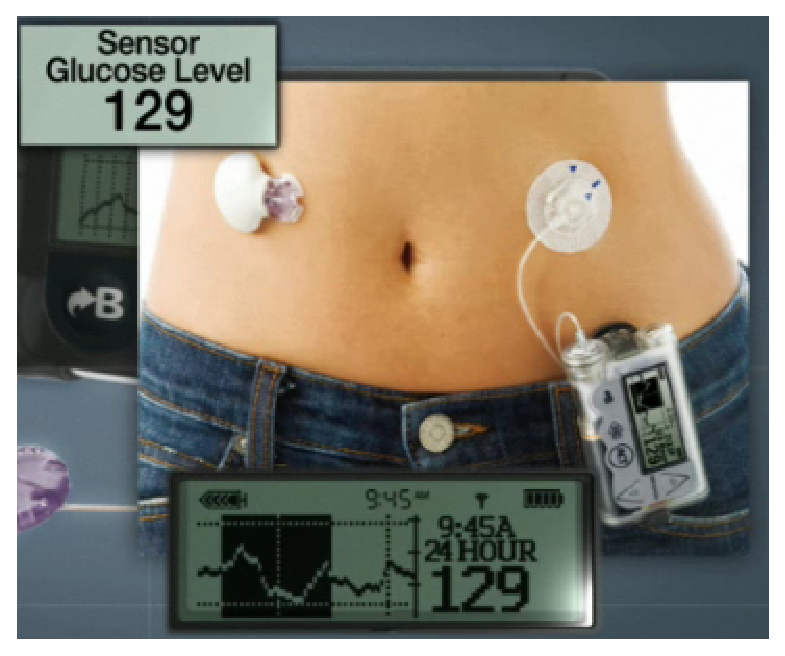
\includegraphics[scale=0.75]{p1.eps}
\caption{Insulin pumps from \cite{hanselman} used with permission from Medtronic Mini-Med, Inc.}
\label{fig:3}
\end{figure}
%\end{figure*}

\section{Security Issues in IMDs}
\label{sec:2}

With the rise in use of IMDs, security becomes a critical issue, as attacks on IMDs
may do harm to the patient \cite{Safety}. There are a couple of
attacks that an adversary may launch on IMDs.
For example, pacemakers and implantable cardioverter defibrillator
(ICDs) contain a magnetic switch that is activated by sufficiently
powerful magnetic fields \cite{mag}. The current
magnetic-switch-based access does not require any authentication and
thus is insecure. Vulnerabilities in the communication interface of
wireless programmable IMDs may allow attackers to monitor and alter
the function of medical devices without even being in close proximity
to the patient \cite{Inside}. The consequences of an unprotected IMD
have the potential to be fatal \cite{Panescu}. Kevin Fu et al. launched
an attack against an implantable cardioverter defibrillator using a
software radio to deliver a defibrillation (shock). Similarly, IBM's
Jay Radcliffe presented an attack against insulin pumps in Aug.
2011. Using an easily obtainable USB device, Radcliffe \cite{Radcliffe}
was able to track data transmitted from the computer and control the
insulin pump's operations by intercepting wireless signals sent
between the sensor device and the display device on his BG monitors;
and he could cause them to display inaccurate readings. To launch
this attack, the serial number of the target device must be known
beforehand. In Oct. 2011, McAfee's Barnaby Jack extended Jay's work
and discovered more fatal attacks including disabling the device
alarm and subsequently delivering a lethal dose without knowing the
device's serial number in advance. In addition, IMDs contain sensitive
patient data and information. A health insurance company may be interested
in this kind of data, which could be used to increase patients' health
insurance premium or even deny a patient's request.

% -- This claim seems highly unlikely...the U.S. medical insurance
% -- industry is far too regulated to allow this to occur
%The attacks targeting implantable medical devices may also be launched by
%insurance companies to make more profit.
IMD readers may be installed near the gate of a building by a malicious party, and the readers can harvest privacy
information from patients' IMDs when they walk through the gate. To
sum up, many attacks could be launched on IMDs, and it is critical to provide security and privacy
capabilities to IMDs.

\section{Challenges and Research Issues}
\label{subsec:3}

Securing IMDs is a very challenging task due
to their very limiting resource constraints in terms of energy
supply, processing power, storage space, etc. An IMD is implanted in a patient's body and is expected to operate
for several months or years. Typical IMDs are powered by a non-rechargeable battery, and replacement of the battery requires surgery. Re-charging an IMD via an external RF electromagnetic source causes thermal effects in body tissues and thus is not recommended. 


In this book, we present related works in Chapter 2, which consists
of defense solutions for IMDs in normal situation as well as during emergencies. In Chapter 3, we discuss the Resource Depletion (RD) attacks and a defense scheme based on a patient's IMD access pattern. In Chapter 3, we present a light-weight biometrics based secure access control scheme for IMDs during emergencies. The conclusion and our future directions are given in Chapter 5.

%\input{referenc1}
